\documentclass[1p]{elsarticle_modified}
%\bibliographystyle{elsarticle-num}

%\usepackage[colorlinks]{hyperref}
%\usepackage{abbrmath_seonhwa} %\Abb, \Ascr, \Acal ,\Abf, \Afrak
\usepackage{amsfonts}
\usepackage{amssymb}
\usepackage{amsmath}
\usepackage{amsthm}
\usepackage{scalefnt}
\usepackage{amsbsy}
\usepackage{kotex}
\usepackage{caption}
\usepackage{subfig}
\usepackage{color}
\usepackage{graphicx}
\usepackage{xcolor} %% white, black, red, green, blue, cyan, magenta, yellow
\usepackage{float}
\usepackage{setspace}
\usepackage{hyperref}

\usepackage{tikz}
\usetikzlibrary{arrows}

\usepackage{multirow}
\usepackage{array} % fixed length table
\usepackage{hhline}

%%%%%%%%%%%%%%%%%%%%%
\makeatletter
\renewcommand*\env@matrix[1][\arraystretch]{%
	\edef\arraystretch{#1}%
	\hskip -\arraycolsep
	\let\@ifnextchar\new@ifnextchar
	\array{*\c@MaxMatrixCols c}}
\makeatother %https://tex.stackexchange.com/questions/14071/how-can-i-increase-the-line-spacing-in-a-matrix
%%%%%%%%%%%%%%%

\usepackage[normalem]{ulem}

\newcommand{\msout}[1]{\ifmmode\text{\sout{\ensuremath{#1}}}\else\sout{#1}\fi}
%SOURCE: \msout is \stkout macro in https://tex.stackexchange.com/questions/20609/strikeout-in-math-mode

\newcommand{\cancel}[1]{
	\ifmmode
	{\color{red}\msout{#1}}
	\else
	{\color{red}\sout{#1}}
	\fi
}

\newcommand{\add}[1]{
	{\color{blue}\uwave{#1}}
}

\newcommand{\replace}[2]{
	\ifmmode
	{\color{red}\msout{#1}}{\color{blue}\uwave{#2}}
	\else
	{\color{red}\sout{#1}}{\color{blue}\uwave{#2}}
	\fi
}

\newcommand{\Sol}{\mathcal{S}} %segment
\newcommand{\D}{D} %diagram
\newcommand{\A}{\mathcal{A}} %arc


%%%%%%%%%%%%%%%%%%%%%%%%%%%%%5 test

\def\sl{\operatorname{\textup{SL}}(2,\Cbb)}
\def\psl{\operatorname{\textup{PSL}}(2,\Cbb)}
\def\quan{\mkern 1mu \triangleright \mkern 1mu}

\theoremstyle{definition}
\newtheorem{thm}{Theorem}[section]
\newtheorem{prop}[thm]{Proposition}
\newtheorem{lem}[thm]{Lemma}
\newtheorem{ques}[thm]{Question}
\newtheorem{cor}[thm]{Corollary}
\newtheorem{defn}[thm]{Definition}
\newtheorem{exam}[thm]{Example}
\newtheorem{rmk}[thm]{Remark}
\newtheorem{alg}[thm]{Algorithm}

\newcommand{\I}{\sqrt{-1}}
\begin{document}

%\begin{frontmatter}
%
%\title{Boundary parabolic representations of knots up to 8 crossings}
%
%%% Group authors per affiliation:
%\author{Yunhi Cho} 
%\address{Department of Mathematics, University of Seoul, Seoul, Korea}
%\ead{yhcho@uos.ac.kr}
%
%
%\author{Seonhwa Kim} %\fnref{s_kim}}
%\address{Center for Geometry and Physics, Institute for Basic Science, Pohang, 37673, Korea}
%\ead{ryeona17@ibs.re.kr}
%
%\author{Hyuk Kim}
%\address{Department of Mathematical Sciences, Seoul National University, Seoul 08826, Korea}
%\ead{hyukkim@snu.ac.kr}
%
%\author{Seokbeom Yoon}
%\address{Department of Mathematical Sciences, Seoul National University, Seoul, 08826,  Korea}
%\ead{sbyoon15@snu.ac.kr}
%
%\begin{abstract}
%We find all boundary parabolic representation of knots up to 8 crossings.
%
%\end{abstract}
%\begin{keyword}
%    \MSC[2010] 57M25 
%\end{keyword}
%
%\end{frontmatter}

%\linenumbers
%\tableofcontents
%
\newcommand\colored[1]{\textcolor{white}{\rule[-0.35ex]{0.8em}{1.4ex}}\kern-0.8em\color{red} #1}%
%\newcommand\colored[1]{\textcolor{white}{ #1}\kern-2.17ex	\textcolor{white}{ #1}\kern-1.81ex	\textcolor{white}{ #1}\kern-2.15ex\color{red}#1	}

{\Large $\underline{12a_{0274}~(K12a_{0274})}$}

\setlength{\tabcolsep}{10pt}
\renewcommand{\arraystretch}{1.6}
\vspace{1cm}\begin{tabular}{m{100pt}>{\centering\arraybackslash}m{274pt}}
\multirow{5}{120pt}{
	\centering
	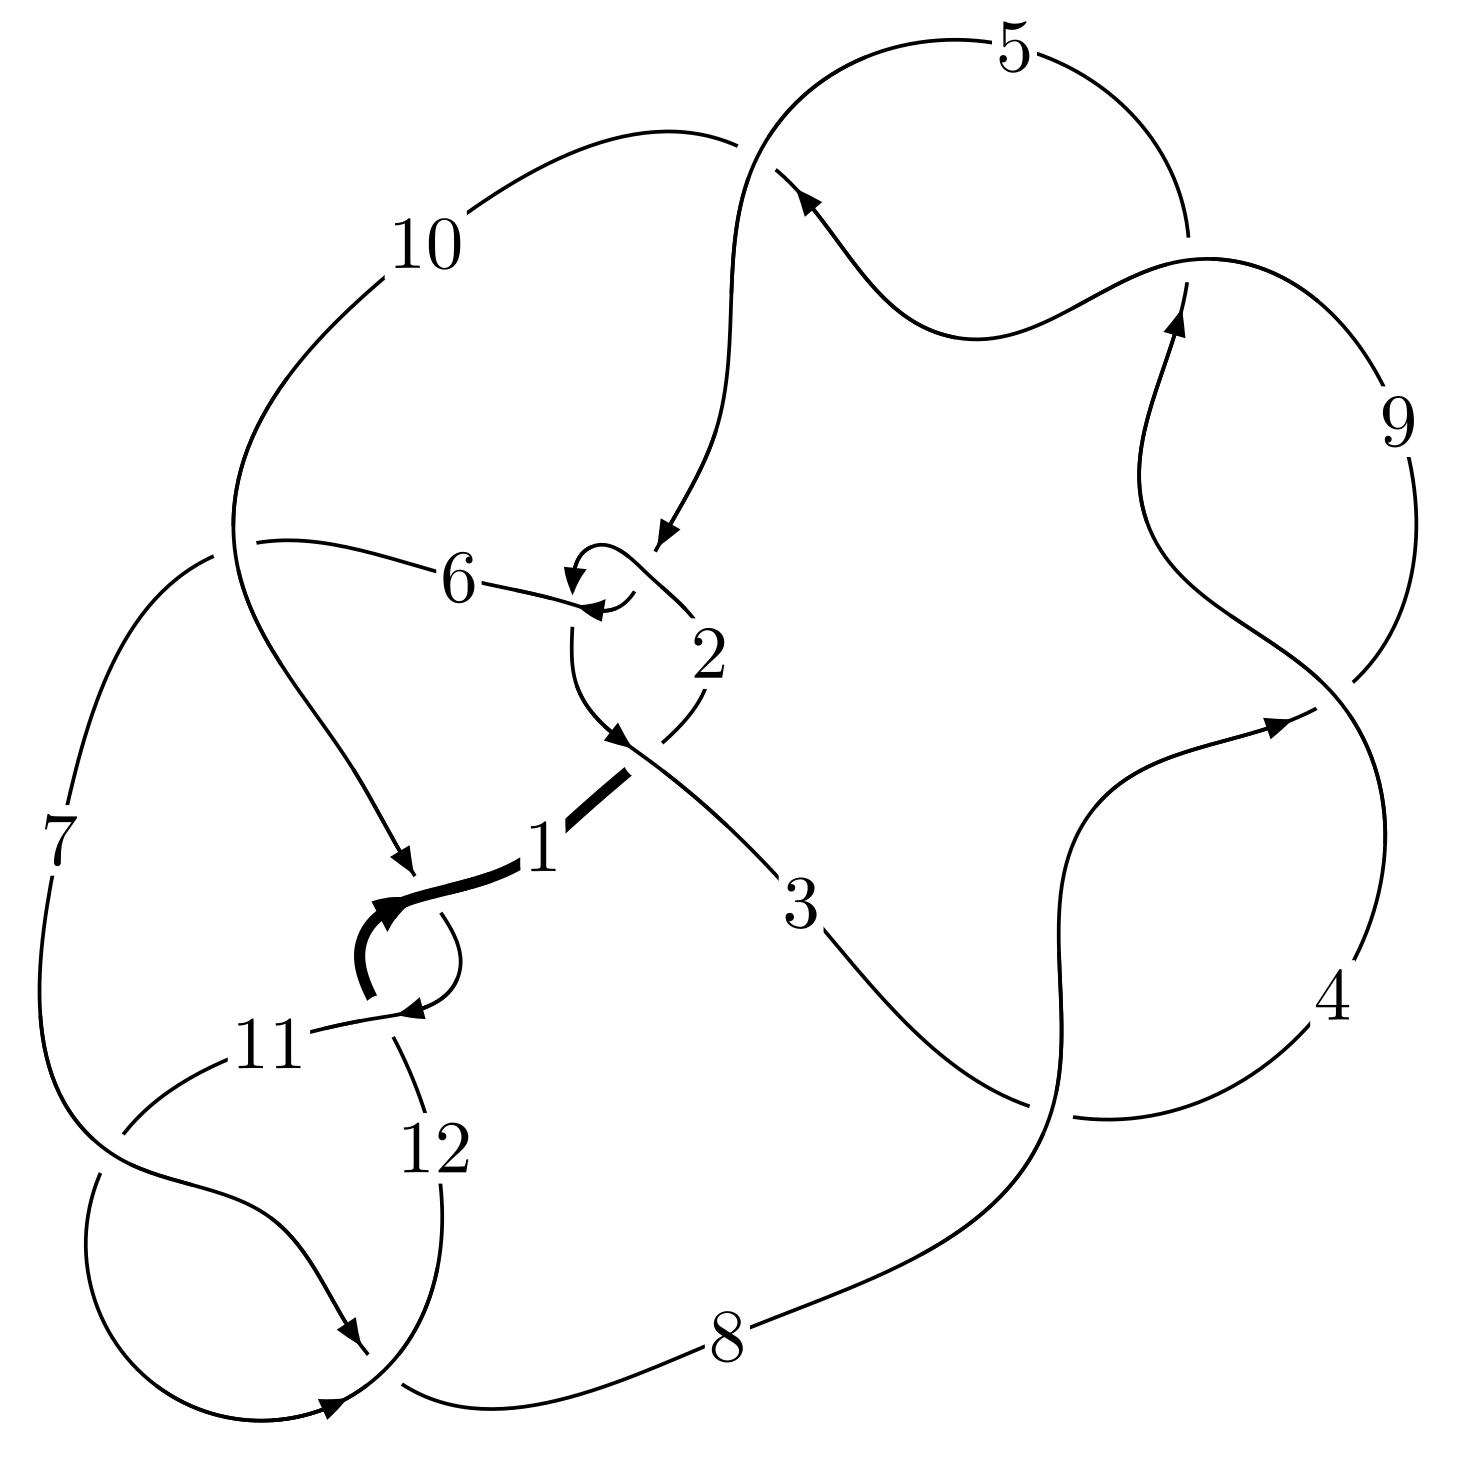
\includegraphics[width=112pt]{../../../GIT/diagram.site/Diagrams/png/1075_12a_0274.png}\\
\ \ \ A knot diagram\footnotemark}&
\allowdisplaybreaks
\textbf{Linearized knot diagam} \\
\cline{2-2}
 &
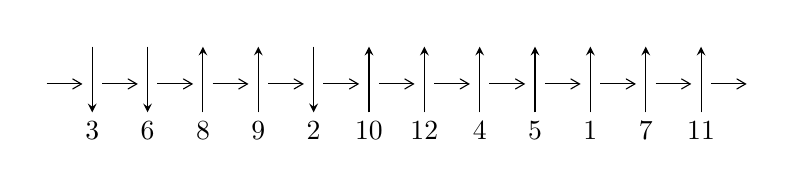
\begin{tikzpicture}[x=20pt, y=17pt]
	% nodes
	\node (C0) at (0, 0) {};
	\node (C1) at (1, 0) {};
	\node (C1U) at (1, +1) {};
	\node (C1D) at (1, -1) {3};

	\node (C2) at (2, 0) {};
	\node (C2U) at (2, +1) {};
	\node (C2D) at (2, -1) {6};

	\node (C3) at (3, 0) {};
	\node (C3U) at (3, +1) {};
	\node (C3D) at (3, -1) {8};

	\node (C4) at (4, 0) {};
	\node (C4U) at (4, +1) {};
	\node (C4D) at (4, -1) {9};

	\node (C5) at (5, 0) {};
	\node (C5U) at (5, +1) {};
	\node (C5D) at (5, -1) {2};

	\node (C6) at (6, 0) {};
	\node (C6U) at (6, +1) {};
	\node (C6D) at (6, -1) {10};

	\node (C7) at (7, 0) {};
	\node (C7U) at (7, +1) {};
	\node (C7D) at (7, -1) {12};

	\node (C8) at (8, 0) {};
	\node (C8U) at (8, +1) {};
	\node (C8D) at (8, -1) {4};

	\node (C9) at (9, 0) {};
	\node (C9U) at (9, +1) {};
	\node (C9D) at (9, -1) {5};

	\node (C10) at (10, 0) {};
	\node (C10U) at (10, +1) {};
	\node (C10D) at (10, -1) {1};

	\node (C11) at (11, 0) {};
	\node (C11U) at (11, +1) {};
	\node (C11D) at (11, -1) {7};

	\node (C12) at (12, 0) {};
	\node (C12U) at (12, +1) {};
	\node (C12D) at (12, -1) {11};
	\node (C13) at (13, 0) {};

	% arrows
	\draw[->,>={angle 60}]
	(C0) edge (C1) (C1) edge (C2) (C2) edge (C3) (C3) edge (C4) (C4) edge (C5) (C5) edge (C6) (C6) edge (C7) (C7) edge (C8) (C8) edge (C9) (C9) edge (C10) (C10) edge (C11) (C11) edge (C12) (C12) edge (C13) ;	\draw[->,>=stealth]
	(C1U) edge (C1D) (C2U) edge (C2D) (C3D) edge (C3U) (C4D) edge (C4U) (C5U) edge (C5D) (C6D) edge (C6U) (C7D) edge (C7U) (C8D) edge (C8U) (C9D) edge (C9U) (C10D) edge (C10U) (C11D) edge (C11U) (C12D) edge (C12U) ;
	\end{tikzpicture} \\
\hhline{~~} \\& 
\textbf{Solving Sequence} \\ \cline{2-2} 
 &
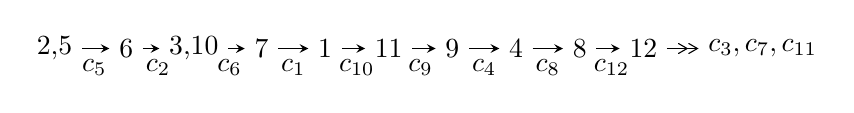
\begin{tikzpicture}[x=23pt, y=7pt]
	% node
	\node (A0) at (-1/8, 0) {2,5};
	\node (A1) at (1, 0) {6};
	\node (A2) at (33/16, 0) {3,10};
	\node (A3) at (25/8, 0) {7};
	\node (A4) at (33/8, 0) {1};
	\node (A5) at (41/8, 0) {11};
	\node (A6) at (49/8, 0) {9};
	\node (A7) at (57/8, 0) {4};
	\node (A8) at (65/8, 0) {8};
	\node (A9) at (73/8, 0) {12};
	\node (C1) at (1/2, -1) {$c_{5}$};
	\node (C2) at (3/2, -1) {$c_{2}$};
	\node (C3) at (21/8, -1) {$c_{6}$};
	\node (C4) at (29/8, -1) {$c_{1}$};
	\node (C5) at (37/8, -1) {$c_{10}$};
	\node (C6) at (45/8, -1) {$c_{9}$};
	\node (C7) at (53/8, -1) {$c_{4}$};
	\node (C8) at (61/8, -1) {$c_{8}$};
	\node (C9) at (69/8, -1) {$c_{12}$};
	\node (A10) at (11, 0) {$c_{3},c_{7},c_{11}$};

	% edge
	\draw[->,>=stealth]	
	(A0) edge (A1) (A1) edge (A2) (A2) edge (A3) (A3) edge (A4) (A4) edge (A5) (A5) edge (A6) (A6) edge (A7) (A7) edge (A8) (A8) edge (A9) ;
	\draw[->>,>={angle 60}]	
	(A9) edge (A10);
\end{tikzpicture} \\ 

\end{tabular} \\

\footnotetext{
The image of knot diagram is generated by the software ``\textbf{Draw programme}" developed by Andrew Bartholomew(\url{http://www.layer8.co.uk/maths/draw/index.htm\#Running-draw}), where we modified some parts for our purpose(\url{https://github.com/CATsTAILs/LinksPainter}).
}\phantom \\ \newline 
\centering \textbf{Ideals for irreducible components\footnotemark of $X_{\text{par}}$} 
 
\begin{align*}
I^u_{1}&=\langle 
-2.74822\times10^{78} u^{76}-6.58436\times10^{78} u^{75}+\cdots+3.26649\times10^{78} b-2.45503\times10^{79},\\
\phantom{I^u_{1}}&\phantom{= \langle  }3.83245\times10^{80} u^{76}+1.21540\times10^{81} u^{75}+\cdots+1.50259\times10^{80} a+7.16663\times10^{81},\;u^{77}+4 u^{76}+\cdots-83 u+23\rangle \\
I^u_{2}&=\langle 
b,\;a^3- a^2+2 a-1,\;u+1\rangle \\
I^u_{3}&=\langle 
-58 a^5-93 a^4+166 a^3+145 a^2+1375 b-1557 a-761,\;a^6+2 a^5- a^4-2 a^3+14 a^2+16 a-23,\;u-1\rangle \\
\\
\end{align*}
\raggedright * 3 irreducible components of $\dim_{\mathbb{C}}=0$, with total 86 representations.\\
\footnotetext{All coefficients of polynomials are rational numbers. But the coefficients are sometimes approximated in decimal forms when there is not enough margin.}
\newpage
\renewcommand{\arraystretch}{1}
\centering \section*{I. $I^u_{1}= \langle -2.75\times10^{78} u^{76}-6.58\times10^{78} u^{75}+\cdots+3.27\times10^{78} b-2.46\times10^{79},\;3.83\times10^{80} u^{76}+1.22\times10^{81} u^{75}+\cdots+1.50\times10^{80} a+7.17\times10^{81},\;u^{77}+4 u^{76}+\cdots-83 u+23 \rangle$}
\flushleft \textbf{(i) Arc colorings}\\
\begin{tabular}{m{7pt} m{180pt} m{7pt} m{180pt} }
\flushright $a_{2}=$&$\begin{pmatrix}0\\u\end{pmatrix}$ \\
\flushright $a_{5}=$&$\begin{pmatrix}1\\0\end{pmatrix}$ \\
\flushright $a_{6}=$&$\begin{pmatrix}1\\u^2\end{pmatrix}$ \\
\flushright $a_{3}=$&$\begin{pmatrix}- u\\- u^3+u\end{pmatrix}$ \\
\flushright $a_{10}=$&$\begin{pmatrix}-2.55057 u^{76}-8.08869 u^{75}+\cdots+198.750 u-47.6953\\0.841338 u^{76}+2.01573 u^{75}+\cdots-6.68307 u+7.51581\end{pmatrix}$ \\
\flushright $a_{7}=$&$\begin{pmatrix}0.0655842 u^{76}-0.348936 u^{75}+\cdots+48.3109 u-3.54945\\0.0711030 u^{76}+0.423687 u^{75}+\cdots-38.3393 u+8.52212\end{pmatrix}$ \\
\flushright $a_{1}=$&$\begin{pmatrix}u^3\\u^5- u^3+u\end{pmatrix}$ \\
\flushright $a_{11}=$&$\begin{pmatrix}-3.33726 u^{76}-10.1169 u^{75}+\cdots+200.943 u-51.1967\\0.855842 u^{76}+2.09894 u^{75}+\cdots-11.7733 u+8.37597\end{pmatrix}$ \\
\flushright $a_{9}=$&$\begin{pmatrix}-3.39191 u^{76}-10.1044 u^{75}+\cdots+205.433 u-55.2111\\0.841338 u^{76}+2.01573 u^{75}+\cdots-6.68307 u+7.51581\end{pmatrix}$ \\
\flushright $a_{4}=$&$\begin{pmatrix}0.874063 u^{76}+3.35873 u^{75}+\cdots-110.479 u+22.8121\\-0.662021 u^{76}-2.14455 u^{75}+\cdots+63.8417 u-16.9405\end{pmatrix}$ \\
\flushright $a_{8}=$&$\begin{pmatrix}3.78999 u^{76}+11.7097 u^{75}+\cdots-255.675 u+57.5747\\-1.08746 u^{76}-2.22875 u^{75}+\cdots-36.8047 u+1.34287\end{pmatrix}$ \\
\flushright $a_{12}=$&$\begin{pmatrix}0.300634 u^{76}+0.554541 u^{75}+\cdots+21.2154 u-0.921596\\-0.0330706 u^{76}+0.409257 u^{75}+\cdots-65.3295 u+13.9071\end{pmatrix}$\\&\end{tabular}
\flushleft \textbf{(ii) Obstruction class $= -1$}\\~\\
\flushleft \textbf{(iii) Cusp Shapes $= 2.17395 u^{76}+8.19414 u^{75}+\cdots-265.163 u+68.6829$}\\~\\
\newpage\renewcommand{\arraystretch}{1}
\flushleft \textbf{(iv) u-Polynomials at the component}\newline \\
\begin{tabular}{m{50pt}|m{274pt}}
Crossings & \hspace{64pt}u-Polynomials at each crossing \\
\hline $$\begin{aligned}c_{1}\end{aligned}$$&$\begin{aligned}
&u^{77}+36 u^{76}+\cdots+18067 u+529
\end{aligned}$\\
\hline $$\begin{aligned}c_{2},c_{5}\end{aligned}$$&$\begin{aligned}
&u^{77}+4 u^{76}+\cdots-83 u+23
\end{aligned}$\\
\hline $$\begin{aligned}c_{3},c_{4},c_{8}\\c_{9}\end{aligned}$$&$\begin{aligned}
&u^{77}+u^{76}+\cdots+40 u-8
\end{aligned}$\\
\hline $$\begin{aligned}c_{6}\end{aligned}$$&$\begin{aligned}
&u^{77}-2 u^{76}+\cdots+15744 u+1429
\end{aligned}$\\
\hline $$\begin{aligned}c_{7},c_{11}\end{aligned}$$&$\begin{aligned}
&u^{77}+2 u^{76}+\cdots+8 u+1
\end{aligned}$\\
\hline $$\begin{aligned}c_{10},c_{12}\end{aligned}$$&$\begin{aligned}
&u^{77}-26 u^{76}+\cdots+52 u-1
\end{aligned}$\\
\hline
\end{tabular}\\~\\
\newpage\renewcommand{\arraystretch}{1}
\flushleft \textbf{(v) Riley Polynomials at the component}\newline \\
\begin{tabular}{m{50pt}|m{274pt}}
Crossings & \hspace{64pt}Riley Polynomials at each crossing \\
\hline $$\begin{aligned}c_{1}\end{aligned}$$&$\begin{aligned}
&y^{77}+20 y^{76}+\cdots+58766823 y-279841
\end{aligned}$\\
\hline $$\begin{aligned}c_{2},c_{5}\end{aligned}$$&$\begin{aligned}
&y^{77}-36 y^{76}+\cdots+18067 y-529
\end{aligned}$\\
\hline $$\begin{aligned}c_{3},c_{4},c_{8}\\c_{9}\end{aligned}$$&$\begin{aligned}
&y^{77}-91 y^{76}+\cdots+1600 y-64
\end{aligned}$\\
\hline $$\begin{aligned}c_{6}\end{aligned}$$&$\begin{aligned}
&y^{77}-18 y^{76}+\cdots+161870600 y-2042041
\end{aligned}$\\
\hline $$\begin{aligned}c_{7},c_{11}\end{aligned}$$&$\begin{aligned}
&y^{77}-26 y^{76}+\cdots+52 y-1
\end{aligned}$\\
\hline $$\begin{aligned}c_{10},c_{12}\end{aligned}$$&$\begin{aligned}
&y^{77}+54 y^{76}+\cdots+1876 y-1
\end{aligned}$\\
\hline
\end{tabular}\\~\\
\newpage\flushleft \textbf{(vi) Complex Volumes and Cusp Shapes}
$$\begin{array}{c|c|c}  
\text{Solutions to }I^u_{1}& \I (\text{vol} + \sqrt{-1}CS) & \text{Cusp shape}\\
 \hline 
\begin{aligned}
u &= \phantom{-}0.909672 + 0.421724 I \\
a &= \phantom{-}1.145770 - 0.117310 I \\
b &= \phantom{-}1.316650 + 0.146721 I\end{aligned}
 & \phantom{-}1.44070 + 0.67158 I & \phantom{-0.000000 } 0 \\ \hline\begin{aligned}
u &= \phantom{-}0.909672 - 0.421724 I \\
a &= \phantom{-}1.145770 + 0.117310 I \\
b &= \phantom{-}1.316650 - 0.146721 I\end{aligned}
 & \phantom{-}1.44070 - 0.67158 I & \phantom{-0.000000 } 0 \\ \hline\begin{aligned}
u &= \phantom{-}0.958740 + 0.259334 I \\
a &= -1.02808 - 1.54394 I \\
b &= \phantom{-}0.436907 - 0.282220 I\end{aligned}
 & -4.69950 + 2.00322 I & \phantom{-0.000000 } 0 \\ \hline\begin{aligned}
u &= \phantom{-}0.958740 - 0.259334 I \\
a &= -1.02808 + 1.54394 I \\
b &= \phantom{-}0.436907 + 0.282220 I\end{aligned}
 & -4.69950 - 2.00322 I & \phantom{-0.000000 } 0 \\ \hline\begin{aligned}
u &= -0.406477 + 0.928601 I \\
a &= \phantom{-}0.445300 + 0.285962 I \\
b &= -1.61605 + 0.12297 I\end{aligned}
 & \phantom{-}7.99937 - 3.55322 I & \phantom{-0.000000 } 0 \\ \hline\begin{aligned}
u &= -0.406477 - 0.928601 I \\
a &= \phantom{-}0.445300 - 0.285962 I \\
b &= -1.61605 - 0.12297 I\end{aligned}
 & \phantom{-}7.99937 + 3.55322 I & \phantom{-0.000000 } 0 \\ \hline\begin{aligned}
u &= -0.836156 + 0.510128 I \\
a &= \phantom{-}1.39187 - 1.92431 I \\
b &= -1.54628 - 0.04973 I\end{aligned}
 & \phantom{-}2.10806 - 0.97873 I & \phantom{-0.000000 } 0 \\ \hline\begin{aligned}
u &= -0.836156 - 0.510128 I \\
a &= \phantom{-}1.39187 + 1.92431 I \\
b &= -1.54628 + 0.04973 I\end{aligned}
 & \phantom{-}2.10806 + 0.97873 I & \phantom{-0.000000 } 0 \\ \hline\begin{aligned}
u &= -0.846089 + 0.570762 I \\
a &= \phantom{-}0.455833 - 1.127310 I \\
b &= \phantom{-}0.119346 - 0.679087 I\end{aligned}
 & \phantom{-}2.27118 + 2.27901 I & \phantom{-0.000000 } 0 \\ \hline\begin{aligned}
u &= -0.846089 - 0.570762 I \\
a &= \phantom{-}0.455833 + 1.127310 I \\
b &= \phantom{-}0.119346 + 0.679087 I\end{aligned}
 & \phantom{-}2.27118 - 2.27901 I & \phantom{-0.000000 } 0\\
 \hline 
 \end{array}$$\newpage$$\begin{array}{c|c|c}  
\text{Solutions to }I^u_{1}& \I (\text{vol} + \sqrt{-1}CS) & \text{Cusp shape}\\
 \hline 
\begin{aligned}
u &= -0.597501 + 0.832618 I \\
a &= \phantom{-}0.671200 - 0.276505 I \\
b &= -1.62202 + 0.04903 I\end{aligned}
 & \phantom{-}9.40242 - 0.58348 I & \phantom{-0.000000 } 0 \\ \hline\begin{aligned}
u &= -0.597501 - 0.832618 I \\
a &= \phantom{-}0.671200 + 0.276505 I \\
b &= -1.62202 - 0.04903 I\end{aligned}
 & \phantom{-}9.40242 + 0.58348 I & \phantom{-0.000000 } 0 \\ \hline\begin{aligned}
u &= \phantom{-}0.802252 + 0.545356 I \\
a &= -0.874362 + 0.161172 I \\
b &= -1.201920 - 0.173318 I\end{aligned}
 & \phantom{-}2.10589 - 4.47726 I & \phantom{-0.000000 } 0 \\ \hline\begin{aligned}
u &= \phantom{-}0.802252 - 0.545356 I \\
a &= -0.874362 - 0.161172 I \\
b &= -1.201920 + 0.173318 I\end{aligned}
 & \phantom{-}2.10589 + 4.47726 I & \phantom{-0.000000 } 0 \\ \hline\begin{aligned}
u &= -0.890705 + 0.520123 I \\
a &= -1.08169 + 2.10827 I \\
b &= \phantom{-}1.54943 + 0.06669 I\end{aligned}
 & \phantom{-}1.91630 + 5.14719 I & \phantom{-0.000000 } 0 \\ \hline\begin{aligned}
u &= -0.890705 - 0.520123 I \\
a &= -1.08169 - 2.10827 I \\
b &= \phantom{-}1.54943 - 0.06669 I\end{aligned}
 & \phantom{-}1.91630 - 5.14719 I & \phantom{-0.000000 } 0 \\ \hline\begin{aligned}
u &= \phantom{-}0.991337 + 0.301788 I \\
a &= \phantom{-}0.82004 + 1.60677 I \\
b &= -0.462524 + 0.336790 I\end{aligned}
 & -4.95823 - 3.85716 I & \phantom{-0.000000 } 0 \\ \hline\begin{aligned}
u &= \phantom{-}0.991337 - 0.301788 I \\
a &= \phantom{-}0.82004 - 1.60677 I \\
b &= -0.462524 - 0.336790 I\end{aligned}
 & -4.95823 + 3.85716 I & \phantom{-0.000000 } 0 \\ \hline\begin{aligned}
u &= \phantom{-}0.836998 + 0.614038 I \\
a &= -0.041166 - 1.187280 I \\
b &= \phantom{-}0.857804 - 0.340914 I\end{aligned}
 & \phantom{-}1.92653 - 0.25220 I & \phantom{-0.000000 } 0 \\ \hline\begin{aligned}
u &= \phantom{-}0.836998 - 0.614038 I \\
a &= -0.041166 + 1.187280 I \\
b &= \phantom{-}0.857804 + 0.340914 I\end{aligned}
 & \phantom{-}1.92653 + 0.25220 I & \phantom{-0.000000 } 0\\
 \hline 
 \end{array}$$\newpage$$\begin{array}{c|c|c}  
\text{Solutions to }I^u_{1}& \I (\text{vol} + \sqrt{-1}CS) & \text{Cusp shape}\\
 \hline 
\begin{aligned}
u &= -0.890297 + 0.288879 I \\
a &= -0.425721 + 0.887659 I \\
b &= -0.165105 + 0.473169 I\end{aligned}
 & -1.49628 + 1.00710 I & \phantom{-0.000000 } 0 \\ \hline\begin{aligned}
u &= -0.890297 - 0.288879 I \\
a &= -0.425721 - 0.887659 I \\
b &= -0.165105 - 0.473169 I\end{aligned}
 & -1.49628 - 1.00710 I & \phantom{-0.000000 } 0 \\ \hline\begin{aligned}
u &= -0.400975 + 0.987005 I \\
a &= -0.303931 - 0.289012 I \\
b &= \phantom{-}1.63234 - 0.13703 I\end{aligned}
 & \phantom{-}9.29601 - 9.22325 I & \phantom{-0.000000 } 0 \\ \hline\begin{aligned}
u &= -0.400975 - 0.987005 I \\
a &= -0.303931 + 0.289012 I \\
b &= \phantom{-}1.63234 + 0.13703 I\end{aligned}
 & \phantom{-}9.29601 + 9.22325 I & \phantom{-0.000000 } 0 \\ \hline\begin{aligned}
u &= \phantom{-}1.06557\phantom{ +0.000000I} \\
a &= \phantom{-}1.39720\phantom{ +0.000000I} \\
b &= \phantom{-}1.43866\phantom{ +0.000000I}\end{aligned}
 & \phantom{-}3.34047\phantom{ +0.000000I} & \phantom{-0.000000 } 0 \\ \hline\begin{aligned}
u &= \phantom{-}0.418780 + 0.816135 I \\
a &= -0.148801 - 0.514697 I \\
b &= -0.782315 - 0.480447 I\end{aligned}
 & \phantom{-}1.05052 + 6.88705 I & \phantom{-}9.76091 - 6.50910 I \\ \hline\begin{aligned}
u &= \phantom{-}0.418780 - 0.816135 I \\
a &= -0.148801 + 0.514697 I \\
b &= -0.782315 + 0.480447 I\end{aligned}
 & \phantom{-}1.05052 - 6.88705 I & \phantom{-}9.76091 + 6.50910 I \\ \hline\begin{aligned}
u &= \phantom{-}0.573921 + 0.715342 I \\
a &= -0.261874 - 0.208626 I \\
b &= -0.895579 - 0.336201 I\end{aligned}
 & \phantom{-}5.54189 + 1.10408 I & \phantom{-}15.4148 - 1.4693 I \\ \hline\begin{aligned}
u &= \phantom{-}0.573921 - 0.715342 I \\
a &= -0.261874 + 0.208626 I \\
b &= -0.895579 + 0.336201 I\end{aligned}
 & \phantom{-}5.54189 - 1.10408 I & \phantom{-}15.4148 + 1.4693 I \\ \hline\begin{aligned}
u &= -0.540901 + 0.962764 I \\
a &= -0.345496 + 0.047931 I \\
b &= \phantom{-}1.65287 - 0.08862 I\end{aligned}
 & \phantom{-}14.3060 - 2.7130 I & \phantom{-0.000000 } 0\\
 \hline 
 \end{array}$$\newpage$$\begin{array}{c|c|c}  
\text{Solutions to }I^u_{1}& \I (\text{vol} + \sqrt{-1}CS) & \text{Cusp shape}\\
 \hline 
\begin{aligned}
u &= -0.540901 - 0.962764 I \\
a &= -0.345496 - 0.047931 I \\
b &= \phantom{-}1.65287 + 0.08862 I\end{aligned}
 & \phantom{-}14.3060 + 2.7130 I & \phantom{-0.000000 } 0 \\ \hline\begin{aligned}
u &= \phantom{-}0.970781 + 0.539274 I \\
a &= \phantom{-}0.23436 + 1.40764 I \\
b &= -0.708068 + 0.428688 I\end{aligned}
 & \phantom{-}0.09329 - 4.18401 I & \phantom{-0.000000 } 0 \\ \hline\begin{aligned}
u &= \phantom{-}0.970781 - 0.539274 I \\
a &= \phantom{-}0.23436 - 1.40764 I \\
b &= -0.708068 - 0.428688 I\end{aligned}
 & \phantom{-}0.09329 + 4.18401 I & \phantom{-0.000000 } 0 \\ \hline\begin{aligned}
u &= -0.695841 + 0.894243 I \\
a &= -0.401450 + 0.493510 I \\
b &= \phantom{-}1.65626 - 0.02689 I\end{aligned}
 & \phantom{-}11.38460 + 4.14926 I & \phantom{-0.000000 } 0 \\ \hline\begin{aligned}
u &= -0.695841 - 0.894243 I \\
a &= -0.401450 - 0.493510 I \\
b &= \phantom{-}1.65626 + 0.02689 I\end{aligned}
 & \phantom{-}11.38460 - 4.14926 I & \phantom{-0.000000 } 0 \\ \hline\begin{aligned}
u &= \phantom{-}0.643060 + 0.568525 I \\
a &= -0.462709 + 0.784941 I \\
b &= -1.075780 + 0.071760 I\end{aligned}
 & \phantom{-}2.18683 - 4.44396 I & \phantom{-}11.04197 + 6.64377 I \\ \hline\begin{aligned}
u &= \phantom{-}0.643060 - 0.568525 I \\
a &= -0.462709 - 0.784941 I \\
b &= -1.075780 - 0.071760 I\end{aligned}
 & \phantom{-}2.18683 + 4.44396 I & \phantom{-}11.04197 - 6.64377 I \\ \hline\begin{aligned}
u &= -1.15096\phantom{ +0.000000I} \\
a &= \phantom{-}0.896231\phantom{ +0.000000I} \\
b &= \phantom{-}0.456757\phantom{ +0.000000I}\end{aligned}
 & -0.0502180\phantom{ +0.000000I} & \phantom{-0.000000 } 0 \\ \hline\begin{aligned}
u &= -1.024390 + 0.528329 I \\
a &= -0.596620 + 1.107350 I \\
b &= -0.262025 + 0.677567 I\end{aligned}
 & -3.39577 + 2.31723 I & \phantom{-0.000000 } 0 \\ \hline\begin{aligned}
u &= -1.024390 - 0.528329 I \\
a &= -0.596620 - 1.107350 I \\
b &= -0.262025 - 0.677567 I\end{aligned}
 & -3.39577 - 2.31723 I & \phantom{-0.000000 } 0\\
 \hline 
 \end{array}$$\newpage$$\begin{array}{c|c|c}  
\text{Solutions to }I^u_{1}& \I (\text{vol} + \sqrt{-1}CS) & \text{Cusp shape}\\
 \hline 
\begin{aligned}
u &= \phantom{-}0.373401 + 0.749056 I \\
a &= \phantom{-}0.027274 + 0.494073 I \\
b &= \phantom{-}0.721323 + 0.440410 I\end{aligned}
 & \phantom{-}0.00960 + 1.45996 I & \phantom{-}7.97618 - 1.67296 I \\ \hline\begin{aligned}
u &= \phantom{-}0.373401 - 0.749056 I \\
a &= \phantom{-}0.027274 - 0.494073 I \\
b &= \phantom{-}0.721323 - 0.440410 I\end{aligned}
 & \phantom{-}0.00960 - 1.45996 I & \phantom{-}7.97618 + 1.67296 I \\ \hline\begin{aligned}
u &= -1.017340 + 0.584382 I \\
a &= \phantom{-}0.580607 - 1.153790 I \\
b &= \phantom{-}0.244773 - 0.720969 I\end{aligned}
 & -2.43522 + 7.84920 I & \phantom{-0.000000 } 0 \\ \hline\begin{aligned}
u &= -1.017340 - 0.584382 I \\
a &= \phantom{-}0.580607 + 1.153790 I \\
b &= \phantom{-}0.244773 + 0.720969 I\end{aligned}
 & -2.43522 - 7.84920 I & \phantom{-0.000000 } 0 \\ \hline\begin{aligned}
u &= -0.550357 + 0.611012 I \\
a &= \phantom{-}0.327725 - 1.139910 I \\
b &= -0.076911 - 0.650916 I\end{aligned}
 & -1.07363 - 3.09170 I & \phantom{-}6.13866 + 1.90820 I \\ \hline\begin{aligned}
u &= -0.550357 - 0.611012 I \\
a &= \phantom{-}0.327725 + 1.139910 I \\
b &= -0.076911 + 0.650916 I\end{aligned}
 & -1.07363 + 3.09170 I & \phantom{-}6.13866 - 1.90820 I \\ \hline\begin{aligned}
u &= \phantom{-}1.013480 + 0.645468 I \\
a &= -0.05966 - 1.47790 I \\
b &= \phantom{-}0.784663 - 0.521607 I\end{aligned}
 & \phantom{-}4.27243 - 6.32707 I & \phantom{-0.000000 } 0 \\ \hline\begin{aligned}
u &= \phantom{-}1.013480 - 0.645468 I \\
a &= -0.05966 + 1.47790 I \\
b &= \phantom{-}0.784663 + 0.521607 I\end{aligned}
 & \phantom{-}4.27243 + 6.32707 I & \phantom{-0.000000 } 0 \\ \hline\begin{aligned}
u &= -1.191670 + 0.202786 I \\
a &= -0.937769 + 0.691714 I \\
b &= -0.500980 + 0.368243 I\end{aligned}
 & -4.82096 + 1.25692 I & \phantom{-0.000000 } 0 \\ \hline\begin{aligned}
u &= -1.191670 - 0.202786 I \\
a &= -0.937769 - 0.691714 I \\
b &= -0.500980 - 0.368243 I\end{aligned}
 & -4.82096 - 1.25692 I & \phantom{-0.000000 } 0\\
 \hline 
 \end{array}$$\newpage$$\begin{array}{c|c|c}  
\text{Solutions to }I^u_{1}& \I (\text{vol} + \sqrt{-1}CS) & \text{Cusp shape}\\
 \hline 
\begin{aligned}
u &= -1.218840 + 0.157900 I \\
a &= \phantom{-}1.046590 - 0.605303 I \\
b &= \phantom{-}0.556485 - 0.309636 I\end{aligned}
 & -4.31085 - 4.23744 I & \phantom{-0.000000 } 0 \\ \hline\begin{aligned}
u &= -1.218840 - 0.157900 I \\
a &= \phantom{-}1.046590 + 0.605303 I \\
b &= \phantom{-}0.556485 + 0.309636 I\end{aligned}
 & -4.31085 + 4.23744 I & \phantom{-0.000000 } 0 \\ \hline\begin{aligned}
u &= \phantom{-}0.590345 + 0.485361 I \\
a &= -0.231755 - 0.263888 I \\
b &= \phantom{-}0.740376 + 0.068232 I\end{aligned}
 & \phantom{-}1.195250 - 0.076686 I & \phantom{-}9.28796 - 0.38114 I \\ \hline\begin{aligned}
u &= \phantom{-}0.590345 - 0.485361 I \\
a &= -0.231755 + 0.263888 I \\
b &= \phantom{-}0.740376 - 0.068232 I\end{aligned}
 & \phantom{-}1.195250 + 0.076686 I & \phantom{-}9.28796 + 0.38114 I \\ \hline\begin{aligned}
u &= -0.994216 + 0.757099 I \\
a &= \phantom{-}0.10861 - 1.43993 I \\
b &= -1.63961 - 0.09571 I\end{aligned}
 & \phantom{-}10.46370 + 1.91251 I & \phantom{-0.000000 } 0 \\ \hline\begin{aligned}
u &= -0.994216 - 0.757099 I \\
a &= \phantom{-}0.10861 + 1.43993 I \\
b &= -1.63961 + 0.09571 I\end{aligned}
 & \phantom{-}10.46370 - 1.91251 I & \phantom{-0.000000 } 0 \\ \hline\begin{aligned}
u &= -1.048280 + 0.682578 I \\
a &= -0.04252 + 1.74716 I \\
b &= \phantom{-}1.61286 + 0.12210 I\end{aligned}
 & \phantom{-}8.02968 + 6.23821 I & \phantom{-0.000000 } 0 \\ \hline\begin{aligned}
u &= -1.048280 - 0.682578 I \\
a &= -0.04252 - 1.74716 I \\
b &= \phantom{-}1.61286 - 0.12210 I\end{aligned}
 & \phantom{-}8.02968 - 6.23821 I & \phantom{-0.000000 } 0 \\ \hline\begin{aligned}
u &= \phantom{-}1.102630 + 0.596774 I \\
a &= \phantom{-}0.11430 + 1.60963 I \\
b &= -0.699462 + 0.578264 I\end{aligned}
 & -2.08597 - 6.55777 I & \phantom{-0.000000 } 0 \\ \hline\begin{aligned}
u &= \phantom{-}1.102630 - 0.596774 I \\
a &= \phantom{-}0.11430 - 1.60963 I \\
b &= -0.699462 - 0.578264 I\end{aligned}
 & -2.08597 + 6.55777 I & \phantom{-0.000000 } 0\\
 \hline 
 \end{array}$$\newpage$$\begin{array}{c|c|c}  
\text{Solutions to }I^u_{1}& \I (\text{vol} + \sqrt{-1}CS) & \text{Cusp shape}\\
 \hline 
\begin{aligned}
u &= \phantom{-}1.114800 + 0.628614 I \\
a &= -0.06903 - 1.61630 I \\
b &= \phantom{-}0.722493 - 0.603009 I\end{aligned}
 & -1.00381 - 12.28950 I & \phantom{-0.000000 } 0 \\ \hline\begin{aligned}
u &= \phantom{-}1.114800 - 0.628614 I \\
a &= -0.06903 + 1.61630 I \\
b &= \phantom{-}0.722493 + 0.603009 I\end{aligned}
 & -1.00381 + 12.28950 I & \phantom{-0.000000 } 0 \\ \hline\begin{aligned}
u &= \phantom{-}1.306230 + 0.170113 I \\
a &= \phantom{-}1.395400 + 0.041474 I \\
b &= \phantom{-}1.54130 + 0.08244 I\end{aligned}
 & \phantom{-}2.08330 + 0.27442 I & \phantom{-0.000000 } 0 \\ \hline\begin{aligned}
u &= \phantom{-}1.306230 - 0.170113 I \\
a &= \phantom{-}1.395400 - 0.041474 I \\
b &= \phantom{-}1.54130 - 0.08244 I\end{aligned}
 & \phantom{-}2.08330 - 0.27442 I & \phantom{-0.000000 } 0 \\ \hline\begin{aligned}
u &= -1.119810 + 0.728835 I \\
a &= -0.22423 - 1.66256 I \\
b &= -1.63651 - 0.15001 I\end{aligned}
 & \phantom{-}12.5328 + 8.8745 I & \phantom{-0.000000 } 0 \\ \hline\begin{aligned}
u &= -1.119810 - 0.728835 I \\
a &= -0.22423 + 1.66256 I \\
b &= -1.63651 + 0.15001 I\end{aligned}
 & \phantom{-}12.5328 - 8.8745 I & \phantom{-0.000000 } 0 \\ \hline\begin{aligned}
u &= -1.164610 + 0.659606 I \\
a &= \phantom{-}0.33637 + 1.89170 I \\
b &= \phantom{-}1.60778 + 0.17375 I\end{aligned}
 & \phantom{-}5.70123 + 9.37064 I & \phantom{-0.000000 } 0 \\ \hline\begin{aligned}
u &= -1.164610 - 0.659606 I \\
a &= \phantom{-}0.33637 - 1.89170 I \\
b &= \phantom{-}1.60778 - 0.17375 I\end{aligned}
 & \phantom{-}5.70123 - 9.37064 I & \phantom{-0.000000 } 0 \\ \hline\begin{aligned}
u &= -0.376520 + 0.530963 I \\
a &= -0.323876 + 1.114950 I \\
b &= \phantom{-}0.156016 + 0.563558 I\end{aligned}
 & -1.67624 + 1.95624 I & \phantom{-}4.81633 - 4.78600 I \\ \hline\begin{aligned}
u &= -0.376520 - 0.530963 I \\
a &= -0.323876 - 1.114950 I \\
b &= \phantom{-}0.156016 - 0.563558 I\end{aligned}
 & -1.67624 - 1.95624 I & \phantom{-}4.81633 + 4.78600 I\\
 \hline 
 \end{array}$$\newpage$$\begin{array}{c|c|c}  
\text{Solutions to }I^u_{1}& \I (\text{vol} + \sqrt{-1}CS) & \text{Cusp shape}\\
 \hline 
\begin{aligned}
u &= \phantom{-}1.36189\phantom{ +0.000000I} \\
a &= -1.42452\phantom{ +0.000000I} \\
b &= -1.57196\phantom{ +0.000000I}\end{aligned}
 & \phantom{-}7.09596\phantom{ +0.000000I} & \phantom{-0.000000 } 0 \\ \hline\begin{aligned}
u &= -1.188130 + 0.675633 I \\
a &= -0.40955 - 1.84238 I \\
b &= -1.61626 - 0.18395 I\end{aligned}
 & \phantom{-}6.8851 + 15.2545 I & \phantom{-0.000000 } 0 \\ \hline\begin{aligned}
u &= -1.188130 - 0.675633 I \\
a &= -0.40955 + 1.84238 I \\
b &= -1.61626 + 0.18395 I\end{aligned}
 & \phantom{-}6.8851 - 15.2545 I & \phantom{-0.000000 } 0 \\ \hline\begin{aligned}
u &= \phantom{-}1.370940 + 0.151238 I \\
a &= -1.41752 - 0.04527 I \\
b &= -1.57417 - 0.07529 I\end{aligned}
 & \phantom{-}3.00302 + 5.57310 I & \phantom{-0.000000 } 0 \\ \hline\begin{aligned}
u &= \phantom{-}1.370940 - 0.151238 I \\
a &= -1.41752 + 0.04527 I \\
b &= -1.57417 + 0.07529 I\end{aligned}
 & \phantom{-}3.00302 - 5.57310 I & \phantom{-0.000000 } 0 \\ \hline\begin{aligned}
u &= \phantom{-}0.510245\phantom{ +0.000000I} \\
a &= -2.32566\phantom{ +0.000000I} \\
b &= -1.33755\phantom{ +0.000000I}\end{aligned}
 & \phantom{-}5.64254\phantom{ +0.000000I} & \phantom{-}18.1120\phantom{ +0.000000I} \\ \hline\begin{aligned}
u &= \phantom{-}0.256713\phantom{ +0.000000I} \\
a &= -1.32663\phantom{ +0.000000I} \\
b &= \phantom{-}0.357915\phantom{ +0.000000I}\end{aligned}
 & \phantom{-}0.734621\phantom{ +0.000000I} & \phantom{-}14.2980\phantom{ +0.000000I}\\
 \hline 
 \end{array}$$\newpage\newpage\renewcommand{\arraystretch}{1}
\centering \section*{II. $I^u_{2}= \langle b,\;a^3- a^2+2 a-1,\;u+1 \rangle$}
\flushleft \textbf{(i) Arc colorings}\\
\begin{tabular}{m{7pt} m{180pt} m{7pt} m{180pt} }
\flushright $a_{2}=$&$\begin{pmatrix}0\\-1\end{pmatrix}$ \\
\flushright $a_{5}=$&$\begin{pmatrix}1\\0\end{pmatrix}$ \\
\flushright $a_{6}=$&$\begin{pmatrix}1\\1\end{pmatrix}$ \\
\flushright $a_{3}=$&$\begin{pmatrix}1\\0\end{pmatrix}$ \\
\flushright $a_{10}=$&$\begin{pmatrix}a\\0\end{pmatrix}$ \\
\flushright $a_{7}=$&$\begin{pmatrix}a^2+1\\1\end{pmatrix}$ \\
\flushright $a_{1}=$&$\begin{pmatrix}-1\\-1\end{pmatrix}$ \\
\flushright $a_{11}=$&$\begin{pmatrix}0\\- a\end{pmatrix}$ \\
\flushright $a_{9}=$&$\begin{pmatrix}a\\0\end{pmatrix}$ \\
\flushright $a_{4}=$&$\begin{pmatrix}1\\0\end{pmatrix}$ \\
\flushright $a_{8}=$&$\begin{pmatrix}a\\0\end{pmatrix}$ \\
\flushright $a_{12}=$&$\begin{pmatrix}-1\\- a^2-1\end{pmatrix}$\\&\end{tabular}
\flushleft \textbf{(ii) Obstruction class $= 1$}\\~\\
\flushleft \textbf{(iii) Cusp Shapes $= -2 a^2-2 a+2$}\\~\\
\newpage\renewcommand{\arraystretch}{1}
\flushleft \textbf{(iv) u-Polynomials at the component}\newline \\
\begin{tabular}{m{50pt}|m{274pt}}
Crossings & \hspace{64pt}u-Polynomials at each crossing \\
\hline $$\begin{aligned}c_{1},c_{2}\end{aligned}$$&$\begin{aligned}
&(u-1)^3
\end{aligned}$\\
\hline $$\begin{aligned}c_{3},c_{4},c_{8}\\c_{9}\end{aligned}$$&$\begin{aligned}
&u^3
\end{aligned}$\\
\hline $$\begin{aligned}c_{5}\end{aligned}$$&$\begin{aligned}
&(u+1)^3
\end{aligned}$\\
\hline $$\begin{aligned}c_{6},c_{10}\end{aligned}$$&$\begin{aligned}
&u^3+u^2+2 u+1
\end{aligned}$\\
\hline $$\begin{aligned}c_{7}\end{aligned}$$&$\begin{aligned}
&u^3- u^2+1
\end{aligned}$\\
\hline $$\begin{aligned}c_{11}\end{aligned}$$&$\begin{aligned}
&u^3+u^2-1
\end{aligned}$\\
\hline $$\begin{aligned}c_{12}\end{aligned}$$&$\begin{aligned}
&u^3- u^2+2 u-1
\end{aligned}$\\
\hline
\end{tabular}\\~\\
\newpage\renewcommand{\arraystretch}{1}
\flushleft \textbf{(v) Riley Polynomials at the component}\newline \\
\begin{tabular}{m{50pt}|m{274pt}}
Crossings & \hspace{64pt}Riley Polynomials at each crossing \\
\hline $$\begin{aligned}c_{1},c_{2},c_{5}\end{aligned}$$&$\begin{aligned}
&(y-1)^3
\end{aligned}$\\
\hline $$\begin{aligned}c_{3},c_{4},c_{8}\\c_{9}\end{aligned}$$&$\begin{aligned}
&y^3
\end{aligned}$\\
\hline $$\begin{aligned}c_{6},c_{10},c_{12}\end{aligned}$$&$\begin{aligned}
&y^3+3 y^2+2 y-1
\end{aligned}$\\
\hline $$\begin{aligned}c_{7},c_{11}\end{aligned}$$&$\begin{aligned}
&y^3- y^2+2 y-1
\end{aligned}$\\
\hline
\end{tabular}\\~\\
\newpage\flushleft \textbf{(vi) Complex Volumes and Cusp Shapes}
$$\begin{array}{c|c|c}  
\text{Solutions to }I^u_{2}& \I (\text{vol} + \sqrt{-1}CS) & \text{Cusp shape}\\
 \hline 
\begin{aligned}
u &= -1.00000\phantom{ +0.000000I} \\
a &= \phantom{-}0.215080 + 1.307140 I \\
b &= \phantom{-0.000000 } 0\end{aligned}
 & -4.66906 + 2.82812 I & \phantom{-}4.89456 - 3.73884 I \\ \hline\begin{aligned}
u &= -1.00000\phantom{ +0.000000I} \\
a &= \phantom{-}0.215080 - 1.307140 I \\
b &= \phantom{-0.000000 } 0\end{aligned}
 & -4.66906 - 2.82812 I & \phantom{-}4.89456 + 3.73884 I \\ \hline\begin{aligned}
u &= -1.00000\phantom{ +0.000000I} \\
a &= \phantom{-}0.569840\phantom{ +0.000000I} \\
b &= \phantom{-0.000000 } 0\end{aligned}
 & -0.531480\phantom{ +0.000000I} & \phantom{-}0.210880\phantom{ +0.000000I}\\
 \hline 
 \end{array}$$\newpage\newpage\renewcommand{\arraystretch}{1}
\centering \section*{III. $I^u_{3}= \langle -58 a^5+1375 b+\cdots-1557 a-761,\;a^6+2 a^5- a^4-2 a^3+14 a^2+16 a-23,\;u-1 \rangle$}
\flushleft \textbf{(i) Arc colorings}\\
\begin{tabular}{m{7pt} m{180pt} m{7pt} m{180pt} }
\flushright $a_{2}=$&$\begin{pmatrix}0\\1\end{pmatrix}$ \\
\flushright $a_{5}=$&$\begin{pmatrix}1\\0\end{pmatrix}$ \\
\flushright $a_{6}=$&$\begin{pmatrix}1\\1\end{pmatrix}$ \\
\flushright $a_{3}=$&$\begin{pmatrix}-1\\0\end{pmatrix}$ \\
\flushright $a_{10}=$&$\begin{pmatrix}a\\0.0421818 a^{5}+0.0676364 a^{4}+\cdots+1.13236 a+0.553455\end{pmatrix}$ \\
\flushright $a_{7}=$&$\begin{pmatrix}0.0167273 a^{5}+0.0785455 a^{4}+\cdots+0.121455 a+0.0298182\\-0.0167273 a^{5}-0.0785455 a^{4}+\cdots-0.121455 a-0.0298182\end{pmatrix}$ \\
\flushright $a_{1}=$&$\begin{pmatrix}1\\1\end{pmatrix}$ \\
\flushright $a_{11}=$&$\begin{pmatrix}0.0421818 a^{5}+0.0676364 a^{4}+\cdots+1.13236 a+0.553455\\0.0843636 a^{5}+0.135273 a^{4}+\cdots+1.26473 a+1.10691\end{pmatrix}$ \\
\flushright $a_{9}=$&$\begin{pmatrix}-0.0421818 a^{5}-0.0676364 a^{4}+\cdots-0.132364 a-0.553455\\0.0421818 a^{5}+0.0676364 a^{4}+\cdots+1.13236 a+0.553455\end{pmatrix}$ \\
\flushright $a_{4}=$&$\begin{pmatrix}-0.0167273 a^{5}-0.0785455 a^{4}+\cdots-0.121455 a-0.0298182\\2\end{pmatrix}$ \\
\flushright $a_{8}=$&$\begin{pmatrix}- a\\-0.0421818 a^{5}-0.0676364 a^{4}+\cdots-1.13236 a-0.553455\end{pmatrix}$ \\
\flushright $a_{12}=$&$\begin{pmatrix}0.0167273 a^{5}+0.0785455 a^{4}+\cdots+0.121455 a+2.02982\\0.0501818 a^{5}+0.235636 a^{4}+\cdots+0.364364 a+2.08945\end{pmatrix}$\\&\end{tabular}
\flushleft \textbf{(ii) Obstruction class $= 1$}\\~\\
\flushleft \textbf{(iii) Cusp Shapes $= -\frac{48}{1375} a^5+\frac{492}{1375} a^4+\frac{896}{1375} a^3+\frac{24}{275} a^2+\frac{608}{1375} a+\frac{13784}{1375}$}\\~\\
\newpage\renewcommand{\arraystretch}{1}
\flushleft \textbf{(iv) u-Polynomials at the component}\newline \\
\begin{tabular}{m{50pt}|m{274pt}}
Crossings & \hspace{64pt}u-Polynomials at each crossing \\
\hline $$\begin{aligned}c_{1},c_{5}\end{aligned}$$&$\begin{aligned}
&(u-1)^6
\end{aligned}$\\
\hline $$\begin{aligned}c_{2}\end{aligned}$$&$\begin{aligned}
&(u+1)^6
\end{aligned}$\\
\hline $$\begin{aligned}c_{3},c_{4},c_{8}\\c_{9}\end{aligned}$$&$\begin{aligned}
&(u^2-2)^3
\end{aligned}$\\
\hline $$\begin{aligned}c_{6},c_{12}\end{aligned}$$&$\begin{aligned}
&(u^3- u^2+2 u-1)^2
\end{aligned}$\\
\hline $$\begin{aligned}c_{7}\end{aligned}$$&$\begin{aligned}
&(u^3+u^2-1)^2
\end{aligned}$\\
\hline $$\begin{aligned}c_{10}\end{aligned}$$&$\begin{aligned}
&(u^3+u^2+2 u+1)^2
\end{aligned}$\\
\hline $$\begin{aligned}c_{11}\end{aligned}$$&$\begin{aligned}
&(u^3- u^2+1)^2
\end{aligned}$\\
\hline
\end{tabular}\\~\\
\newpage\renewcommand{\arraystretch}{1}
\flushleft \textbf{(v) Riley Polynomials at the component}\newline \\
\begin{tabular}{m{50pt}|m{274pt}}
Crossings & \hspace{64pt}Riley Polynomials at each crossing \\
\hline $$\begin{aligned}c_{1},c_{2},c_{5}\end{aligned}$$&$\begin{aligned}
&(y-1)^6
\end{aligned}$\\
\hline $$\begin{aligned}c_{3},c_{4},c_{8}\\c_{9}\end{aligned}$$&$\begin{aligned}
&(y-2)^6
\end{aligned}$\\
\hline $$\begin{aligned}c_{6},c_{10},c_{12}\end{aligned}$$&$\begin{aligned}
&(y^3+3 y^2+2 y-1)^2
\end{aligned}$\\
\hline $$\begin{aligned}c_{7},c_{11}\end{aligned}$$&$\begin{aligned}
&(y^3- y^2+2 y-1)^2
\end{aligned}$\\
\hline
\end{tabular}\\~\\
\newpage\flushleft \textbf{(vi) Complex Volumes and Cusp Shapes}
$$\begin{array}{c|c|c}  
\text{Solutions to }I^u_{3}& \I (\text{vol} + \sqrt{-1}CS) & \text{Cusp shape}\\
 \hline 
\begin{aligned}
u &= \phantom{-}1.00000\phantom{ +0.000000I} \\
a &= \phantom{-}0.844373\phantom{ +0.000000I} \\
b &= \phantom{-}1.41421\phantom{ +0.000000I}\end{aligned}
 & \phantom{-}4.40332\phantom{ +0.000000I} & \phantom{-}11.0200\phantom{ +0.000000I} \\ \hline\begin{aligned}
u &= \phantom{-}1.00000\phantom{ +0.000000I} \\
a &= \phantom{-}1.19913 + 1.30714 I \\
b &= \phantom{-}1.41421\phantom{ +0.000000I}\end{aligned}
 & \phantom{-}0.26574 - 2.82812 I & \phantom{-}4.49024 + 2.97945 I \\ \hline\begin{aligned}
u &= \phantom{-}1.00000\phantom{ +0.000000I} \\
a &= \phantom{-}1.19913 - 1.30714 I \\
b &= \phantom{-}1.41421\phantom{ +0.000000I}\end{aligned}
 & \phantom{-}0.26574 + 2.82812 I & \phantom{-}4.49024 - 2.97945 I \\ \hline\begin{aligned}
u &= \phantom{-}1.00000\phantom{ +0.000000I} \\
a &= -1.98405\phantom{ +0.000000I} \\
b &= -1.41421\phantom{ +0.000000I}\end{aligned}
 & \phantom{-}4.40332\phantom{ +0.000000I} & \phantom{-}11.0200\phantom{ +0.000000I} \\ \hline\begin{aligned}
u &= \phantom{-}1.00000\phantom{ +0.000000I} \\
a &= -1.62929 + 1.30714 I \\
b &= -1.41421\phantom{ +0.000000I}\end{aligned}
 & \phantom{-}0.26574 - 2.82812 I & \phantom{-}4.49024 + 2.97945 I \\ \hline\begin{aligned}
u &= \phantom{-}1.00000\phantom{ +0.000000I} \\
a &= -1.62929 - 1.30714 I \\
b &= -1.41421\phantom{ +0.000000I}\end{aligned}
 & \phantom{-}0.26574 + 2.82812 I & \phantom{-}4.49024 - 2.97945 I\\
 \hline 
 \end{array}$$\newpage
\newpage\renewcommand{\arraystretch}{1}
\centering \section*{ IV. u-Polynomials}
\begin{tabular}{m{50pt}|m{274pt}}
Crossings & \hspace{64pt}u-Polynomials at each crossing \\
\hline $$\begin{aligned}c_{1}\end{aligned}$$&$\begin{aligned}
&((u-1)^9)(u^{77}+36 u^{76}+\cdots+18067 u+529)
\end{aligned}$\\
\hline $$\begin{aligned}c_{2}\end{aligned}$$&$\begin{aligned}
&((u-1)^3)(u+1)^6(u^{77}+4 u^{76}+\cdots-83 u+23)
\end{aligned}$\\
\hline $$\begin{aligned}c_{3},c_{4},c_{8}\\c_{9}\end{aligned}$$&$\begin{aligned}
&u^3(u^2-2)^3(u^{77}+u^{76}+\cdots+40 u-8)
\end{aligned}$\\
\hline $$\begin{aligned}c_{5}\end{aligned}$$&$\begin{aligned}
&((u-1)^6)(u+1)^3(u^{77}+4 u^{76}+\cdots-83 u+23)
\end{aligned}$\\
\hline $$\begin{aligned}c_{6}\end{aligned}$$&$\begin{aligned}
&(u^3- u^2+2 u-1)^2(u^3+u^2+2 u+1)\\
&\cdot(u^{77}-2 u^{76}+\cdots+15744 u+1429)
\end{aligned}$\\
\hline $$\begin{aligned}c_{7}\end{aligned}$$&$\begin{aligned}
&(u^3- u^2+1)(u^3+u^2-1)^2(u^{77}+2 u^{76}+\cdots+8 u+1)
\end{aligned}$\\
\hline $$\begin{aligned}c_{10}\end{aligned}$$&$\begin{aligned}
&((u^3+u^2+2 u+1)^3)(u^{77}-26 u^{76}+\cdots+52 u-1)
\end{aligned}$\\
\hline $$\begin{aligned}c_{11}\end{aligned}$$&$\begin{aligned}
&((u^3- u^2+1)^2)(u^3+u^2-1)(u^{77}+2 u^{76}+\cdots+8 u+1)
\end{aligned}$\\
\hline $$\begin{aligned}c_{12}\end{aligned}$$&$\begin{aligned}
&((u^3- u^2+2 u-1)^3)(u^{77}-26 u^{76}+\cdots+52 u-1)
\end{aligned}$\\
\hline
\end{tabular}\newpage\renewcommand{\arraystretch}{1}
\centering \section*{ V. Riley Polynomials}
\begin{tabular}{m{50pt}|m{274pt}}
Crossings & \hspace{64pt}Riley Polynomials at each crossing \\
\hline $$\begin{aligned}c_{1}\end{aligned}$$&$\begin{aligned}
&((y-1)^9)(y^{77}+20 y^{76}+\cdots+5.87668\times10^{7} y-279841)
\end{aligned}$\\
\hline $$\begin{aligned}c_{2},c_{5}\end{aligned}$$&$\begin{aligned}
&((y-1)^9)(y^{77}-36 y^{76}+\cdots+18067 y-529)
\end{aligned}$\\
\hline $$\begin{aligned}c_{3},c_{4},c_{8}\\c_{9}\end{aligned}$$&$\begin{aligned}
&y^3(y-2)^6(y^{77}-91 y^{76}+\cdots+1600 y-64)
\end{aligned}$\\
\hline $$\begin{aligned}c_{6}\end{aligned}$$&$\begin{aligned}
&((y^3+3 y^2+2 y-1)^3)(y^{77}-18 y^{76}+\cdots+1.61871\times10^{8} y-2042041)
\end{aligned}$\\
\hline $$\begin{aligned}c_{7},c_{11}\end{aligned}$$&$\begin{aligned}
&((y^3- y^2+2 y-1)^3)(y^{77}-26 y^{76}+\cdots+52 y-1)
\end{aligned}$\\
\hline $$\begin{aligned}c_{10},c_{12}\end{aligned}$$&$\begin{aligned}
&((y^3+3 y^2+2 y-1)^3)(y^{77}+54 y^{76}+\cdots+1876 y-1)
\end{aligned}$\\
\hline
\end{tabular}
\vskip 2pc
\end{document}